% Lecture Template for ME3050-001-002-Tristan Hill - Spring 2020
% Dynamics Modeling and Controls
% Frequency Response

% I am finally converting my stuff to BEAMER

% Document settings

%\documentclass{beamer}                  % for presentation ?
\documentclass[handout]{beamer}  % for handout ?
\usepackage{beamerthemesplit}
\usepackage{amsmath}
\usepackage{listings}
\usepackage{multicol}
\usepackage{framed}
\usepackage{amssymb}


\lstdefinestyle{myCustomMatlabStyle}{
  language=Matlab,
  numbers=left,
  stepnumber=1,
  numbersep=10pt,
  tabsize=4,
  showspaces=false,
  showstringspaces=false
}
\lstset{basicstyle=\ttfamily\tiny,style=myCustomMatlabStyle}
%lstset{language=MATLAB,basicstyle=\ttfamily\small,showstringspaces=false}



\beamertemplateballitem

\definecolor{TTUpurple}{rgb}{0.3098, 0.1607, 0.5176} % TTU Purple (primary)
\definecolor{TTUgold}{rgb}{1.0000, 0.8666, 0.0000} % TTU Gold (primary)

\setbeamercolor{palette primary}{bg=TTUpurple,fg=TTUgold}
\setbeamercolor{palette secondary}{bg=black,fg=TTUgold}
\setbeamercolor{palette tertiary}{bg=black,fg=TTUpurple}
\setbeamercolor{palette quaternary}{bg=TTUgold,fg=black}
\setbeamercolor{structure}{fg=TTUpurple} % itemize, enumerate, etc
\setbeamercolor{section in toc}{fg=TTUpurple} % TOC sections

%\DeclareSymbolFont{bbold}{U}{bbold}{m}{n}
%\DeclareSymbolFontAlphabet{\mathbbold}{bbold}

%\newcommand{\bbfamily}{\fontencoding{U}\fontfamily{bbold}\selectfont}
%\DeclareMathAlphabet{\mathbbold}{U}{bbold}{m}{n}

%\usefonttheme{professionalfonts}

\newcommand{\vspccc}{\vspace{6mm}\\} % large vertical space
\newcommand{\vspcc}{\vspace{4mm}\\}   % medium vertical space
\newcommand{\vspc}{\vspace{2mm}\\}     % small vertical space

\newcommand{\hspcccc}{\hspace{10mm}} % large horizontal space
\newcommand{\hspccc}{\hspace{6mm}} % large horizontal space
\newcommand{\hspcc}{\hspace{4mm}}   % medium horizontal space
\newcommand{\hspc}{\hspace{2mm}}     % small horizontal space


\newcommand{\LT}{\mathcal{L}} % lagrangian

\newcommand{\LNUM}{4 } %Lecture number 4

\newcommand{\secondtitle}{Resonance}% second line of the title of this presentation , aka the topic of this lecture

\title{Frequency Response - Lecture \LNUM}
\author{ME3050 - Dynamics Modeling and Controls} % original formatting from Mike Renfro, September 21, 2004

\date{April  25, 2020}

\begin{document}

\lstset{language=MATLAB,basicstyle=\ttfamily\small,showstringspaces=false}

% Title page1 
\frame{\titlepage \center\textbf{\secondtitle}\vspcc}


% Section 0: Outline
\frame{

\large \textbf{Lecture \LNUM - \secondtitle} \vspc

 \begin{itemize}

	\item Review 2$^{nd}$ Order Frequency Response \vspc % Section 1: 

	\item The Resonance Phenomenon\vspc % Section 2
	
	\item The Resonance Frequency\vspc %Section 3

	\item MATLAB code for Bode Plots \vspc %Section 3
%\item Graph of Frequency Response in MATLAB\vspace{2mm} % Section 4

\end{itemize}

}


%Section 1: Review 2$^{nd}$ Order Frequency Response
\section{Review 2$^{nd}$ Order Frequency Response}

\subsection{Transfer Function of 2$^{nd}$ Order System}
\frame{
\frametitle{Transfer Function of 2$^{nd}$ Order System}

\scalebox{1}{$m\ddot{x}+c\dot{x}+kx=f(t)$ \hspace{5mm}with\hspace{5mm} $f(t)=Asin(\omega t)$} \vspcc
The transfer function can easily be found by taking the Laplace transform of the equation of motion. \vspcc

\begin{framed}
\scalebox{1}{$T(s)=\frac{X(s)}{F(s)}=\frac{1}{ms^2+cs+k}$ \hspace{5mm} Second Order Transfer Function} \vspc
\end{framed}

The amplitude ratio and phase angle can be found from the transfer function. Think about what $M$ means. \vspc

}


\subsection{Overdamped vs. Underdamped Systems}
\frame{
\frametitle{Overdamped vs. Underdamped Systems}

\small

In an \underline{overdamped} system, both roots are real and distinct.\vspc

\begin{framed}
\scalebox{0.75}{$M\left(\omega\right)=|T\left(j\omega\right)|=\frac{|1/k|}{|\tau_1j\omega+1||\tau_2j\omega+1|}$} \vspc
\scalebox{0.75}{$m\left(\omega\right)=20logM\left(\omega\right)=20log|1/k|-20log|\tau_1\omega j+1|-20log|\tau_2\omega j+1|$}\vspc
\scalebox{0.75}{$\phi\left(\omega\right)=\angle\frac{1}{k}-\angle\left(\tau_1\omega j+1\right)-\angle\left(\tau_2\omega_j+1\right)$}
\end{framed}
In an \underline{underdamped} system, the roots are complex conjugates.\vspc
\begin{framed}
\scalebox{0.75}{$M\left(r\right)=|T\left(r\right)|=\frac{1}{\sqrt{\left(1-r^2\right)^2+\left(2\zeta r\right)^2}}$ \hspc with \hspc$r=\frac{\omega}{\omega_n} $}\vspc
\scalebox{0.75}{$\implies m=20logM=-10log\left[\left(1-r^2\right)^2+\left(2\zeta r\right)^2\right]$} \vspc
\scalebox{0.75}{$\phi=\angle 1 - \angle\left(1-r^2+2\zeta rj\right)\implies \phi=-tan\left(\frac{2\zeta r}{1-r^2}\right)$}\vspc
\end{framed}

}

% Section 2:  The Resonace Phenomenon
\section{The Resonace Phenomenon}
\subsection{The Resonace Spike}
\frame{
\frametitle{The Resonance Spike}

In the underdamped second order system only two regions are present separated by the point near $r=1$. \vspc

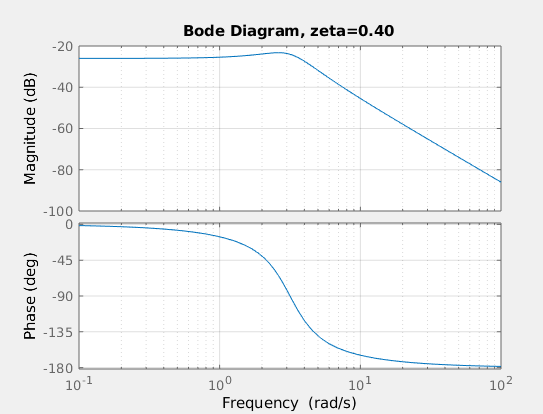
\includegraphics[scale=.18]{lecture4_fig1.png} 
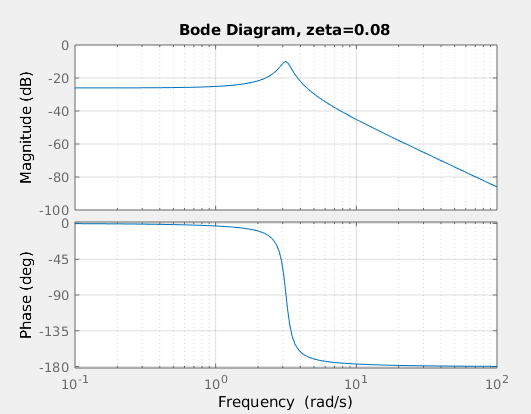
\includegraphics[scale=.18]{lecture4_fig2.png} 
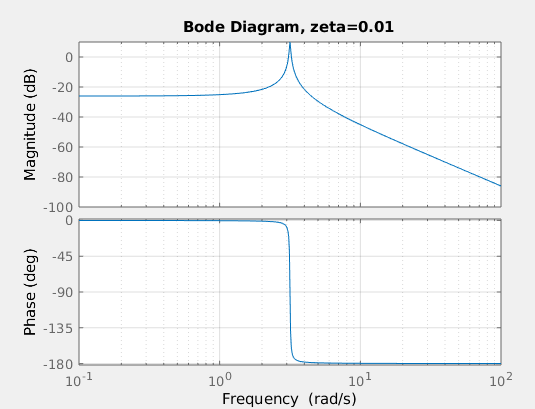
\includegraphics[scale=.18]{lecture4_fig3.png}  \vspc

As the damping ratio decreases something significant happens at this points. Remember, these are graphs of $m=20logM$. \vspc

}

\subsection{The Effects of Resonance}
\frame{
\frametitle{The Effects of Resonance}

\small

Consider the extreme case in the figure shown. What is the physical significance of the values of $m$ near $r=1$?  \vspc
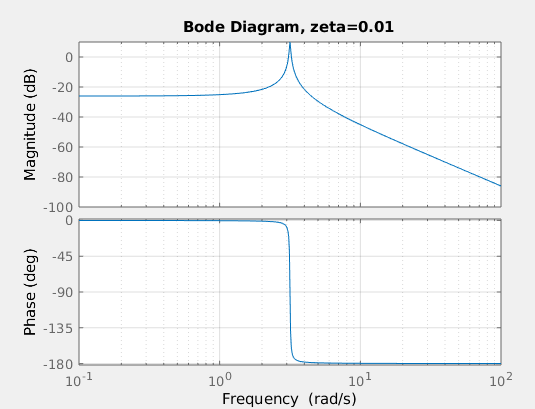
\includegraphics[scale=.25]{lecture4_fig3.png}\hspace{10mm} 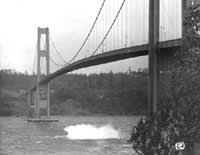
\includegraphics[scale=.6]{galloping_gertie_02.jpg}  \vspc

}


\subsection{Resonance can be Destructive}
\frame{
\frametitle{Resonance can be Destructive}

\small

The resonance peak represents a amplitude  ratio greater than one meaning the output amplitude is larger that in the input amplitude. This large amplitude output displacement caused by resonance correspond to a large force in the spring members and the large forces are transmitted to the body. Large forces cause mechanical failure.

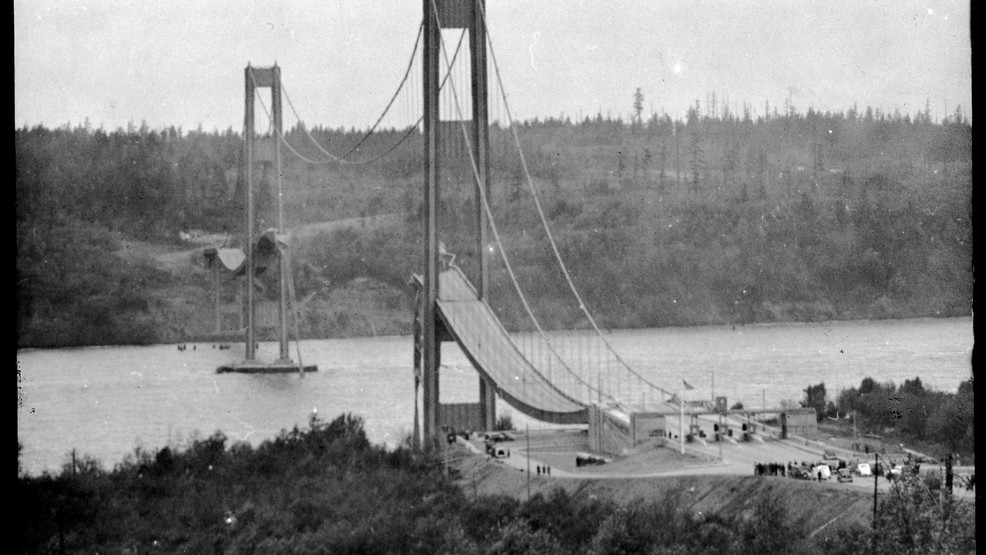
\includegraphics[scale=.20]{galloping_gertie_01.jpg}  \vspc
}



% section 3: The  Resonance Frequency
\frame{
\frametitle{The  Resonance Frequency}

Where on the frequency response graphs does resonance occur? It looks like it is {\it near} $r=1$.\vspc

\scalebox{1}{$M\left(r\right)=\frac{1}{\sqrt{\left(1-r^2\right)^2+\left(2\zeta r\right)^2}}$ \hspc with \hspc$r=\frac{\omega}{\omega_n}$}\vspc

The value of $M$ is maximized when the denominator is minimized. Therefore the resonance frequency is found by taking the derivative of the denominator and setting it equal to zero.  \vspc

\scalebox{1}{$M_{max}$ \hspc occurs at $r=\sqrt{1-2\zeta^2} \implies \omega=\omega_n\sqrt{1-2\zeta^2} $}\vspc

An input frequency equal to the resonance frequency causes maximum output displacement.  \vspc

}

\frame{
\frametitle{The  Resonance Frequency}
The resonance event only occurs in second order systems when the radical shown is positive. This corresponds to systems with damping ratio in the range $0<\zeta< 0.707$ . \vspc

\scalebox{1}{$\omega_r=\omega_n\sqrt{1-2\zeta^2} \hspc 0<\zeta< 0.707$} \vspc

\scalebox{1}{$M_r=\frac{1}{2\zeta\sqrt{1-\zeta^2}}$\hspccc or in decibels\hspccc$m_r=-20log\left(2\zeta\sqrt{1-\zeta^2}\right)$} \vspc

The phase at resonance can also be found. \vspc

\scalebox{1}{$\phi_r=tan^{-1}\left(\frac{\sqrt{1-2\zeta^2}}{\zeta}\right)$}\vspc

}

\frame{
\frametitle{Output Displacement to Input Force}

It is important to note that we multiplied the transfer function by $k$ during the derivations. Therefore if me divide the expressions for $M$ and $M_r$ by $k$ to find the amplitude ratio between input force, $f(t)$ and output displacement, $x_{ss}(t)$\vspc

\scalebox{1}{$M=\frac{1}{k\sqrt{\left(1-r^2\right)^2+\left(2\zeta r\right)^2}}$}\vspc
\scalebox{1}{$\implies \hspcc m=-20log(k)-10log\left[\left(1-r^2\right)^2+\left(2\zeta r\right)^2\right]$}\vspc
\scalebox{1}{$M_r=\frac{1}{k2\zeta\sqrt{1-\zeta^2}}$}\vspc
\scalebox{1}{$\implies \hspcc m_r=-20log\left(k\right)-20log\left(2\zeta\sqrt{1-\zeta^2}\right) $}\vspc

}
% references is not a section for now, for looks and it would be a waste of space
\frame{

\frametitle{References}

\begin{itemize}
	\item System Dynamics, Palm III, Third Edition - Chapter 9 - System Response in the Frequency Domain
\end{itemize}

}

\end{document}









 